\section{KubeEdge}

KubeEdge merupakan solusi \textit{edge architecture} \textit{open source} yang mengembangkan kubernetes secara lebih jauh untuk domain spesifik yaitu \textit{IoT} \parencite{kubeedge}. Arsitektur KubeEdge memungkinkan untuk melakukan konfigurasi perangkat \textit{IoT} yang berada di \textit{edge} secara terpusat melalui komponen \textit{cloud}. Dengan adanya dua komponen \textit{edge core} dan \textit{cloud core} membuat komunikasi antara platform aplikasi menjadi \textit{seamless}.

Untuk menghubungkan \textit{cloud core} dengan \textit{edge core}, KubeEdge menggunakan sebuah \textit{controller} yang dapat melakukan \textit{device discovery} terhadap \textit{edge core}. Setelah \textit{edge core} ditemukan, \textit{controller} akan meneruskan \textit{request} ke komponen berikutnya yaitu Sync Service. KubeEdge menggunakan KubeBus untuk melakukan komunikasi antar \textit{cloud} dan \textit{edge}, KubeBus menggunakan protokol HTTP untuk meneruskan \textit{request} dari \textit{cloud core} menuju \textit{edge core}. Setelah \textit{request} diterima oleh \textit{edge core}, akan digunakan protokol MQTT untuk menerima ataupun mengirim data dari perangkat \textit{IoT} ke \textit{edge core} begitu pula sebaliknya.

\begin{figure}
  \centering
  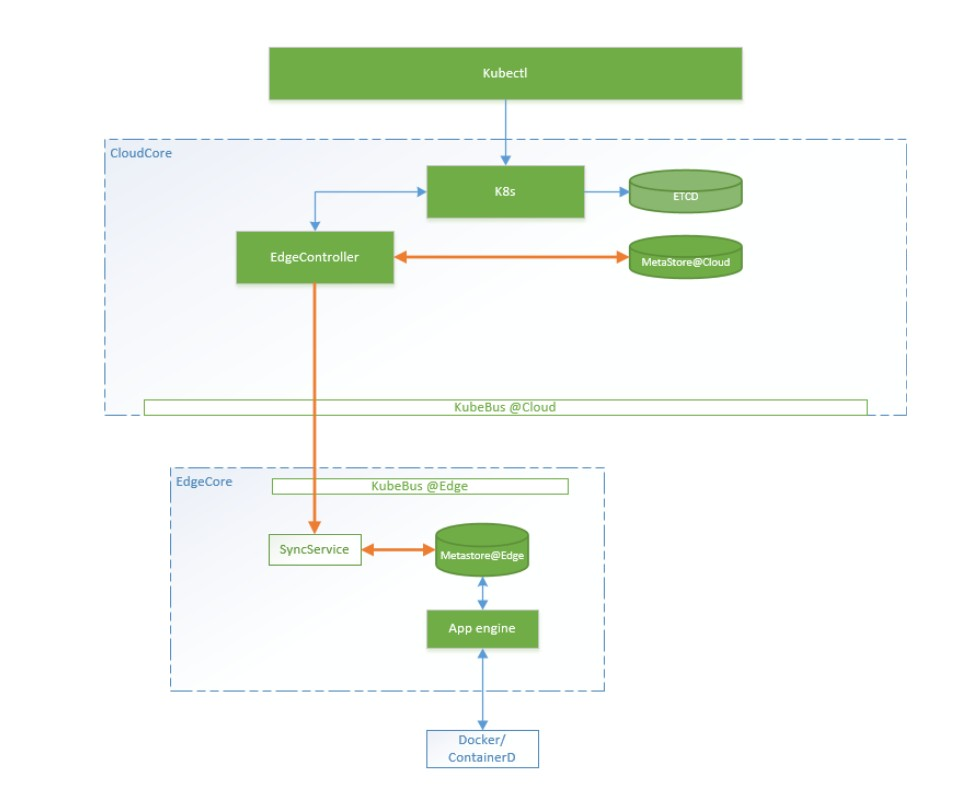
\includegraphics[width=1\textwidth]{resources/chapter-2/arsitektur-kube-edge.jpg}
  \caption{Arsitektur KubeEdge \parencite{kubeedge}}
  \label{fig:arsitektur-kube-edge}
\end{figure}